\documentclass{article}

\usepackage{booktabs}
\usepackage{graphicx}
\usepackage{authblk}
\usepackage{fancyhdr}
\usepackage{datetime}

\title{3P-U -- Debiaising using MICE}
\author[1,2]{\'Emilien ARNAUD}
\author[1]{Daniel Aiham GHAZALI}
\author[2]{Gilles DEQUEN}

\affil[1]{Department of Emergency Medicine, Amiens University Hospital}
\affil[2]{Modelisation, Information and Systems laboratory, Amiens Picardy Jules Vernes University}

\pagestyle{fancy}
\lhead{\'E. ARNAUD and al.}
\rhead{3P-U -- Debiasing using MICE}
\lfoot{Working Paper}
\cfoot{Page \thepage}
\rfoot{\today}

\begin{document}
    \maketitle{}
    \section{Rational}
        The hypothesis is that real measured values contain different biases : measure bias, human reporting biais, \dots

        MICE algorithm imputes missing values based on known values in the dataset. We hypothesize that the generated MICE model used to fill values contains no bias. Then, applying the model on the measured values would improve the model.

    \section{Setup}

        The setup can be run using this command : \texttt{cli.py setup}

        \subsection{Split indexes}

        We take the raw dataset, we random 20\% indexes : the  validation set. The rest is the train set. The validation will only be used to validate our experiments.

        The \texttt{ archived/validation\_indexes.pkl } files stores the validations indexes. The train indexes are rest.


        \subsection{Missing data}

        For both dataset, we store all locations (index, column) were a data is missing

        \subsection{Columns description}

        The experimenter must define in \texttt{ archived/columns\_description.py } two variables to correctly type the dataframe columns:

        \begin{enumerate}
            \item \texttt{cols\_categorical}: List of columns that should be considered as categorical
            \item \texttt{cols\_numerical}: List of columns that should be considered as numerical
        \end{enumerate}

    \section{Protocole}
        \subsection{First setup}
            We begin to launch the setup command

        \subsection{Frist train of the raw data with no modification}
            We train a reference model on the train data.
            This is the base model. All other models will be trained using the same method to be compared.
            The generated model is presented \textbf{raw} in Figure \ref{fig:all_models}

            \begin{enumerate}
                \item We load split dataset
                \item We train a model on the training dataset
                \item We compute the AUC on the validation dataset
            \end{enumerate}

        \subsection{Training MICE}
            \begin{enumerate}
                \item We train MICE on training dataset only.
                \item We replace missing values in both dataset
                \item We generated a model which is presented \textbf{mice} in Figure \ref{fig:all_models}
            \end{enumerate}


        \subsection{Replace non missing data}

            Here, we replace the non missing data by imputed data. We exclude from this treatment the target column and columns were all data were filled, since the completion model will not work. 

            Excluded variables from being debiased are : CIMU, AGE, SEXE, HOSPITALISATION, HEURE\_ARRIVEE, JOUR\_SEMAINE, MOIS, SEMAINE\_ANNEE, main complaint one hot encoded
            
            \subsubsection{Delta between datasets}
                We compute the delta of the values $\Delta = V_{mesured} - V_{imputed}$. The differences are presented in Table \ref{tab:delta}

                \textbf{Question : how can we measure the delta for categorical variables ?}

                \begin{table*}
                    \centering
                    \begin{tabular}{lllll}
                        \toprule
                        Variable & Min & Mean & Std & Max \\
                        \midrule
                        CETONEMIE & -16 & -0.0033 & 0.37 & 127 \\
                        DOULEUR & -10 & -0.09 & 3.41 & 10 \\
                        FC & -170 & 0.09 & 21.72 & 188 \\
                        GLYCEMIE & -102 & -0.27 & 3.28 & 496 \\
                        HEMOCUE & -12.98 & -0.00 & 0.56 & 13.55 \\
                        OH & -8.32 & -0.00 & 0.16 & 7.62 \\
                        OXYGENE & -126 & -0.04 & 3.38 & 126 \\
                        PAD & -935 & 0.24 & 28.21 & 928 \\
                        PAS & -217 & 0.28 & 27.14 & 200 \\
                        SATURATION & -45 & 0.02 & 2.60 & 44 \\
                        TEMPERATURE& -37.6 & -0.00 & 0.90 & 9.20 \\
                        \bottomrule
                    \end{tabular}
                    \caption{Difference between the dataset filled by MICE and the dataset filled and corrected by MICE.}
                    \label{tab:delta}
                \end{table*}
            
                \subsubsection{Model}
                The generated model is presented \textbf{mice\_corrected} in Figure \ref{fig:all_models}

        \subsection{Using deep learning}
            We trained a models using deep learning rather than XGBoost to see if the type of evaluation model is dependent to the MICE and correction.

            \subsubsection{For the raw dataset}
                To use deep learning method, we must fill all missing values, then we used mean for numerical variables and mode for categorical variables.
                The generated model is presented \textbf{deep\_raw} in Figure \ref{fig:all_models}

            \subsubsection{For the MICE dataset}
                We trained a deep model with no modification of the MICED dataset. The generated model is presented \textbf{deep\_mice} in Figure \ref{fig:all_models}

            \subsubsection{For the MICE corrected dataset}
                We trained a deep model with no modification of the MICE corrected dataset. 
                The generated model is presented \textbf{deep\_mice\_corrected} in Figure \ref{fig:all_models}

        \subsection{Comparing all models}
            We put all AUC on the same chart in Figure \ref{fig:all_models}
            \begin{figure*}
                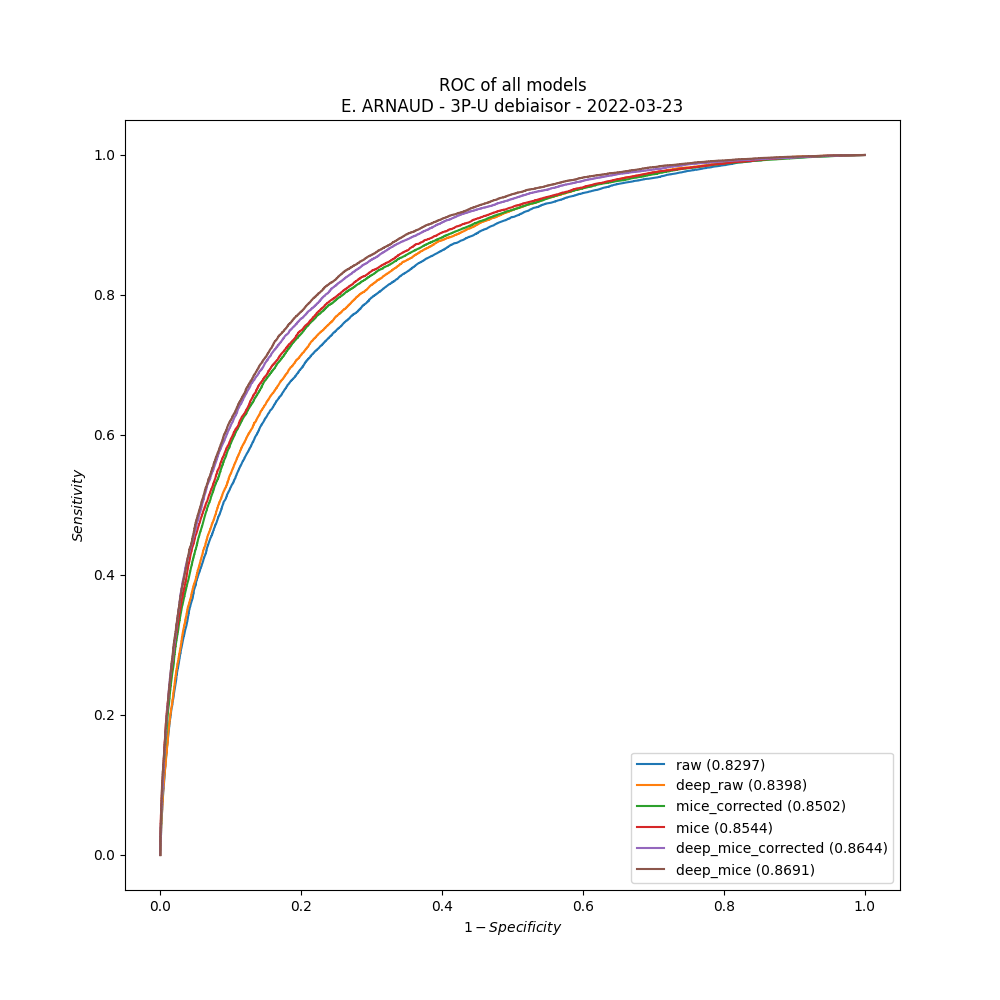
\includegraphics[width=\textwidth]{../archived/all_models.png}
                \caption{AUROC of the models in differents stage of the pipe line. All models starting with \texttt{deep\_} refer to a deep learning model, others refer to an XGBoost model.}
                \label{fig:all_models}
            \end{figure*}

\end{document}
